\section{Approach}
\label{approach}

In our initial prototype, replicas are distributed
synchronously to ensure reliability. Our model comprises a
block-level, distributed caching system where unwritten,
dirty data is replicated across the caches of other
clients in the system. We use iSCSI as our cooperative
caching protocol, to make clients in the network aware of
the cache capacity of their peers and utilize any available
free storage to propagate replicas of dirty data. In the
future, we would
like to consider the tradeoff between free space and the
degree of replication in our prototype, so that each client
has a fair chance to replicate their data whenever there is
an update.

% for later: how do clients know where each replica is stored?
% hint: use an in-memory table, generate an unique key from
% bio information, and find replicas in hash table

\subsection{Design}

In our design, we assign a cache partition for holding
replicas from other clients. Device Mapper Cache then
uses the partition as a replica cache, where replicas
are sent to it by a peer client through TCP/IP and given
a time stamp to ensure consistency, since consistency
cannot be guaranteed, especially when not all of the
replica clients respond to a 
replication request.
We define a \textit{captured page} to be
a dirty page belonging to another client. The
\textit{degree of replication} is equivalent to the number
of captured pages in a client. A
\textit{replica target} is a client with enough
free space in its local cache to satisfy
a replication request. Clients replicate data proactively
in the background. During propagation, write
operations are queued until each replica reaches its
replica target.

% COMMENT: We should specify in the section below (or as
% separate section later ) that this is done by a heartbeat
%  monitor daemon. 
A timeout is specified in order to
avoid blocking the writes for too long. The timeout, which
indicates a target failure, is based on the network
latency and can be adjusted depending on network traffic.
We also use a "heartbeat" daemon to immediately flush the
dirty data when the client holding the original data fails.
The daemon works as follows: the replicator client will
synchronize with target clients so that at fixed time
intervals, the target will read a message passed through
TCP indicating that the replicator client is running and that
its cache is available. If either of these conditions fail,
the data is immediately flushed back by the replica client,
chosen from a list of clients with the most up-to-date copy
in order to ensure consistency.

%monitors the activity of the replicator client.

% We need to revise the paragraph below based on our final
% findings.
%%%%%%%%In our evaluation of reliability, we consider different
%%%%%%%%approaches for handling a timeout due to failure,
%%%%%%%%including power failure, node failure, disk failure or
%%%%%%%%failure due to network partition. We analyze various
%%%%%%%%design tradeoffs for failure handling, exploring whether
%%%%%%%%or not writing back to a RAID on the storage server makes
%%%%%%%%the system more reliable than having multiple attempts
%%%%%%%%to replicate the data.

In our evaluation of reliability, we consider different
approaches for handling failure, including power failure,
node failure, disk failure or failure due to network partition.
We analyze various design tradeoffs for failure handling, exploring
whether or not writing back to a RAID on the storage server makes
the system more reliable than having multiple attempts to
replicate the data.

If time allows, our design will include a cache
partitioning algorithm that considers the tradeoff between
free space and the \textit{degree of replication} in each
client in order to perform fair replication across clients,
and ensure system-wide reliability. The benefit for
choosing a replication candidate with enough free space is
as follows:

\begin{equation}
	benefit=\frac{f_i}{r_i}
\end{equation}

where $f_i$
is the free space in node i, and $r_i$ is the degree
of replication in node i. Dynamic network joins and exits
will not be considered for this paper. Therefore, we will
use a circle of peer clients for our initial prototype.
We will also partition the cache of each client so that
a small percentage is allocated to the replicas of its
peers, leaving the implementation of an intelligent
cache partitioning algorithm for future work. 

% COMMENT: Paste figure in this part of the paper. Make it so that it
% covers about a fourth of page, or even a third. 

Figure~\ref{fig:framework} shows the general structure of our prototype.
In our framework a node can serve any of the following roles:
replicator, replica target, or storage server. The sections
below explain each of these roles.

\subsubsection{Storage Server}
\begin{figure*}[t]
  \centering 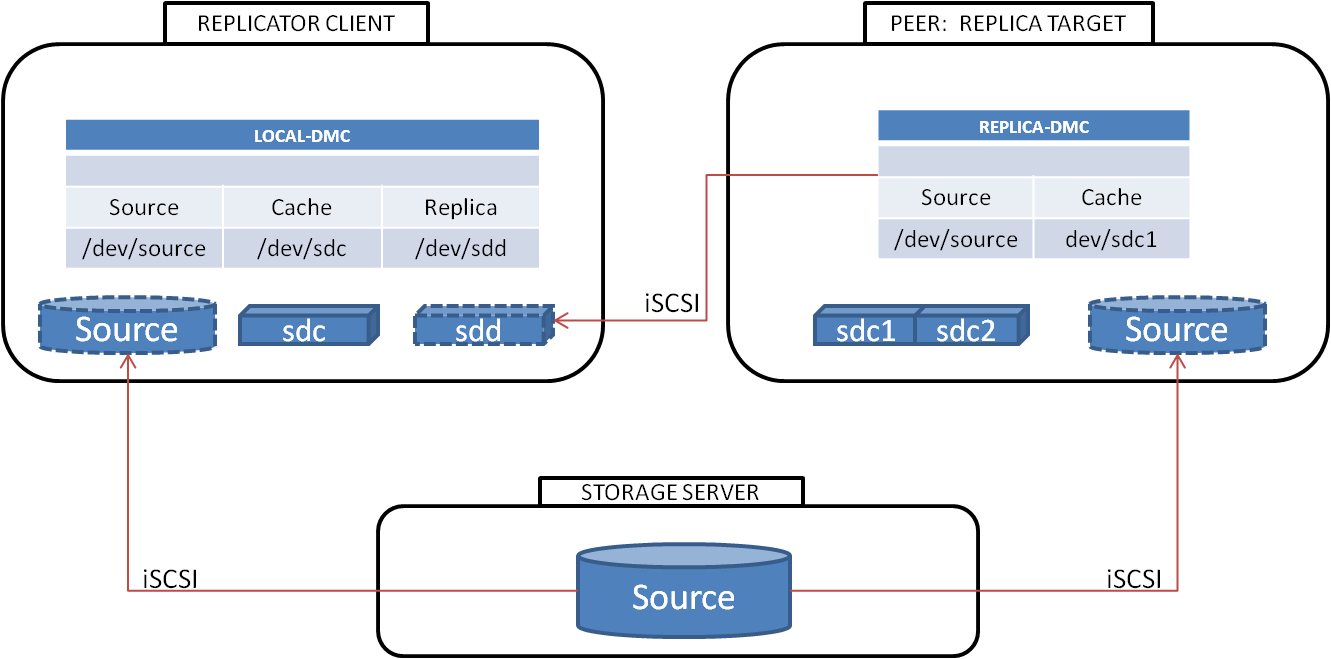
\includegraphics[width=\linewidth]{os_graph.png}
  \caption{The general structure of our prototype. A node can serve
	   any of the following roles: replicator, replica target, or storage
	   server.}
  \label{fig:framework}
\end{figure*}

A storage server node in our system is the machine that holds
the primary storage medium used by the storage area network.
This storage is made available to to other client machines by
way of an IP-based protocol, such as iSCSI. For our prototype
the storage server node provides a source storage device to
both the replicator client and the replica peer target by using
the iSCSI protocol. The replicator and replica target see a 
logical version of the source device and can operate on it just
as it if were physically attached.

\subsubsection{Replica Target}

A replica target node is a client that shares its local SSD
cache device with other clients. This client has two special
functionalities. The first functionality is to handle the copies
of dirty data that are sent to it by other clients who wish
to use it as a recipient for their replicas. The second 
functionality is to serve as a potential source of data recovery
in case the client with the original data fails. The mechanism
used to accomplish these two functionalities is done by 
implementing a special version of the DM Cache module which has
been modified to hold replicas from other clients, and to flush
the versions of dirty data in a recovery scenario. The reason
we use a special version of DM Cache in the peer client
is because it provides us with a logical device which we can
present to the replicator client as a cache device specifically
for replicas. The replicator client can see this device as a local
device by using a protocol like iSCSI. More details
of the implemention of this DM Cache module can be seen in the
implementation section of this paper.

\subsubsection{Replicator}

A replicator node is a client that wishes to replicate its dirty
writes onto other peer clients. This client runs a special version
of DM Cache which allows it to specify a replica cache device,
a local cache device, and source device when loading. The current 
version that we implemented for our prototype only allows it to 
specify a single replica cache device, however, this feature can 
be simply expanded so that when loading our version of DM-Cache on
a client machine, it will have the chance to specify a circle of 
peer cache devices to which it can propagate replicas.
A \textit{circle} 
would just be a group of clients which have agreed to let another
peer client use its free cache space. 


\subsubsection{Communication Protocol}

In order to propagate dirty writes to other peer clients a 
replicator client performs write operations in a replica 
cache device, in addition to the local cache device. This replica
cache device is the virtual block device made available through iSCSI
and it is generated by the replica version of DM Cache running in the
peer client.

The replicator client and the replica target only
need to set up an iSCSI initiator module and an iSCSI target,
respectively. This mechanism allows to transfer data from one client 
to another without having to modify much of the DM Cache source code
and makes it simple to propagate replicas of dirty data to other
devices, whether physical or logical. When a propagation
request is activated, a client will send out a request to
each client in its circle and if not enough clients respond with a
confirmation, it can be assumed that there was not enough free space,
or that there was a failure in some of the clients.

The reason for replicating in a static fashion rather than dynamic is
because we first want to focus on creating
a communication channel that is stable and that has acceptable performance
in comparison to the baseline case. If time allows it, a best-case scenario
implementation will result in a system allowing a client to join a network of
cooperative clients without having to reload DM-Cache with a new circle of clients,
as well as using the intelligent paritioning algorithm discussed earlier.

\subsection{Implementation}

The implementation of our prototype will use DM Cache,
which is an existing block-level caching solution. We will
modify it to incorporate our cooperative caching and
replication mechanisms. The current implementation of
DM-Cache exists as a Linux kernel module. It intercepts
block I/O requests directed towards the main storage device,
and redirects these towards a cache device. Information
about redirected requests, such as source device to cache
device block mappings, block status flags, and other
related meta-data is kept in a special data structure. Our
prototype will use DM-Cache, its block request mapping and
its redirection mechanism as the foundation of
the block-level cache management mechanism.

As part of this project, iSCSI is used as the storage
communications
protocol for DM Cache. In the current setup of DM Cache,
where clients work in a non-cooperative manner, the storage
server functions as the iSCSI target, and the client machine
functions as the iSCSI initiator. In other words, the client
machine would only access the storage resources allocated to
it in the server. In order to transfer blocks of data from
client to client, the new system will require that all
clients have access to the cache of their peers. Having
communication established among peer clients, each client can
then initiate replication processes or act as
target for replicas.

The sections below explain in further detail the implementation
of the replication, communication, and recovery mechanisms
that were implemented as part of this project.

\subsubsection{Replication}
%	NEED TO REVISE THIS TO FIT OUR FINAL WORK
% This will grow as I explain the mechanism I used regarding
% all dm-xxx functions to propagate data from one client to
% another.
Our prototype depends on two special versions of DM Cache 
in order to perform the replication and storage of dirty data.
The first version of DM Cache that we worked on was the one
that replicated data for dirty writes. We will refer to this 
version as "propagator-dmc".

The original version of DM Cache allows one to specify a source
device and local cache device. In our modified version one
can specify a third device which we will refer to as the replica
cache device. This device is just the logical representation of
the device which is made available using iSCSI, and it's 
produced by the replica version of DM Cache running in the peer
client. The advantage of using this method to propagate data 
for dirty writes is that there needs to be little modification
on the DM Cache source code. This is because DM Cache uses a 
special function from the Device-Mapper function library. The
function is dm\_io(). This function allows DM Cache to perform
read or write operations synchronously or asynchronously. 
One special function which we took advantage of is that this
function these services allows us to take a write bio request and
redirect it to more than one block device. All we need to specify
for each destination is the block device, the address, and the 
size of the request. The synchronous function will block until
a request has  been dispatched to both devices. The asynchronous
version allows us to specify a callback function to handle
the completion of both devices, so it does not block.

Besides the block device, the difference between data going to 
the local cache and the replica cache is the address to which
they're directed. For local caches, the "propagator-dmc" version
of DM Cache directs a write request to a section in the local
cache device that is specified by the current cache management
policy (the default configuration we used is based on a 
set-associative cache). As for the replica cache device, the 
address of the request is the same as the original bio request. 
This is done so that when this request is received by the 
replica client it stores a mapping for the original address,
the one pointing to the source device. In the case of
recoveries, the dirty data is flushed to the source device
using this address.

The "propagator-dmc" version handles the two cases in which
a write request in DM Cache results in dirty writes. The first 
case is when a request results in a cache hit. The second one
is when a request results in a cache write miss. In both of these
cases, "propagator-dmc" replicates the dirty data to both 
the local cache device and the replica cache device. In addition,
to handling the cases where dirty data is produced, 
"propagator-dmc" must also handle cases when dirty data is flushed
to the source device and is made clean (valid). Luckily, DM Cache
handles these cases by using a function called write\_back(). 
This function simply copies dirty blocks to the corresponding
address in the source device. For our project we modified it
so that it would also send a modified bio to the replica cache
device when a writeback operation occurred. This modified bio 
contained a special flag, signalling that the data for this 
block was no longer dirty.

%%%%%%%%------- THERE'S STILL SOME WORK 
%%%%%%%%TO DO IN THIS PART OF THE PROJECT, AS OUR IMPLEMENTATION DOES 
%%%%%%%%NOT WORK CORRECTLY, YET ----------------------------------.

\subsubsection{Replica Management}

The second type of DM Cache that we worked on this project
was the version that is in charge of running on the peer 
client that stores the replicas. We will refer to this version
as the "replica-dmc" version. The main function of this
version of DM Cache is in managing the copies of the dirty
data from other clients. For our project, we modified DM Cache
so as to produce a version that can handle the replicas for
only one client per instance.  In order to handle the replicas 
from other clients another instance of "replica-dmc" would have 
to be loaded. When loading this version of DM Cache, the 
parameters we pass are the source device of the replicator 
client, and the partition of the peer's SSD cache device.
Figure~\ref{fig:frameworkd} illustrates how this works.

The first characteristic of this version of DM Cache is
that it is only used to hold dirty data from another client, 
and it's not designed to be used for reading or for 
mounting. In order to make it do this, the cache\_map
function of DM Cache is modified to ignore any read bios,
so that only mappings for dirty writes are stored. 
Currently we used DM Cache's internal structure to store
the mapping between the original bio's source address
and the replica cache address.

%%%%%%%%--------- THE APPROPRIATE
%%%%%%%%WAY TO DO THIS IS TO USE ANOTHER MAPPING STRUCTURE,
%%%%%%%%ONE THAT WOULD ALLOW FOR ALL THE AVAILABLE CACHE SPACE TO
%%%%%%%%BE USED INSTEAD OF SUFFERING FROM THE ISSUES OF A HASH
%%%%%%%%TABLE --------

The second characteristic of the "replica-dmc" version of
DM Cache is that it should discard any data for blocks
that are no longer dirty on the replicator client-side.
This is done by checking for hints on specially-marked bios
coming from the replicator client. Basically, any bio that
is received in the cache\_map function is checked to see
if a special flag has been set by the replicator client. 
Any bio that has this flag set is sent to a function that 
changes the mapping for that block from a dirty state to 
a valid state, that way this mapping is ignored for 
recovery purposes or is replaced if space for a new mapping
is needed.

%%%%%%%%----- ONCE AGAIN WE STILL NEED TO DO WORK
%%%%%%%%TO GET THIS FUNCTION WORKING, SPECIFICALLY WE NEED TO
%%%%%%%%CREATE A MORE STABLE MAPPING STRUCTURE ------

\subsubsection{ Recovery: Heartbeat Daemon}

The heartbeat daemon has a client component that runs on
"propagator-dmc". The client component is a kernel thread
that generates a message at fixed time intervals. The
message is sent only if the replicator has not failed, and
if the local cache of the replicator is available. The
"replica-dmc" uses a web server that expects a \textit{pulse}
from the "propagator-dmc" after a fixed amount of time plus
a reasonable amount of network delay. If the replica client
does not recieve a message from the replicator, then it can
be assumed that the replicator, which originally contained
the data, failed unexpectedly.

The "replica-dmc" includes a mechanism for consulting with
other neighboring caches, to see which one contains the 
most up-to-date copy of the data, in order to maintain
consistency, by writing back the latest replica, in the advent
that not all replica clients received the latest copy
on the update that occured just before the failure. This
mechanism includes metadata about each block, with a time
stamp that is written on each commit and hashed by sector
number.

When a failure occurs, after bootup, the kernel module
will be loaded, along with the circle of clients. The module
will warm the cache from the data stored in the storage server
disk, since the data would have
been flushed immediately after the failure from a replica client
with the most up-to-date copy of the data.

